\documentclass[a4paper, twocolumn]{article}
\usepackage[pdftex, hidelinks]{hyperref}

\usepackage{bm}
\usepackage[T1]{fontenc}
\usepackage[utf8]{inputenc}
\usepackage{algorithmic}
\usepackage{algorithm}
\usepackage{amsfonts}
\usepackage{amssymb}
\usepackage{courier}
\usepackage{booktabs}
\usepackage{graphicx}
\usepackage{listings}
\usepackage{mathtools}
\usepackage{amssymb}
\lstset{basicstyle=\footnotesize\ttfamily,
        breakatwhitespace = false,
        breaklines = true,
        keepspaces = true,
        language = R,
        showspaces = false,
        showstringspaces = false,
        belowcaptionskip = \bigskipamount,
        framerule = 0.80pt,
        frame = tb,
        belowskip = \bigskipamount,
        escapeinside={<@}{@>}}

\title{TDDE01 -- Machine Learning \\
       Group 9 Laboration Report 2}
\author{{Martin Estgren \texttt{<mares480>}} \\
        {Erik S. V. Jansson \texttt{<erija578>}} \\
        {Sebastian Maghsoudi \texttt{<sebma654>}} \\~\\
        {Linköping University (LiU), Sweden}}

\begin{document}
    \pagenumbering{arabic}
    \maketitle % Generate.

    \section*{Assignment 1}

        In this assignment we were tasked with finding the best \emph{feature selection} using \emph{k-fold cross-validation} with \emph{linear regression} as estimator.

        \subsection*{Feature Selection}

        The purpose of this algorithm is to find the subset of features from a given dataset that yields the lowest \emph{cross-validation score}. This is performed by iterating through all possible combinations of features, in this case, \emph{brute forcing} through all possibilities.
        \begin{equation}
            s \in \{1,...,n\}\\
        \end{equation}
        \begin{equation}
            \mathbf{A} = \{s_1,s_2,...,s_{2^n-1}\}\\
        \end{equation}
        \begin{equation}
            \bigcap_{i = 1}^{|\mathbf{A}|}{(s_i)} = \emptyset
        \end{equation}

        \subsection*{K-Fold Cross-Validation}

            The algorithm (as can be seen in \ref{alg:kfoldcv}) splits the given dataset into \( K \) disjoint subsets of equal size, \( K \) is arbitrarily defined as 5 for this assignment. The algorithm then iterates through all the subsets (folds) using the current fold as validation data and all the other folds as training data for the linear regression model.

            \begin{algorithm}
                \caption{K-Fold Cross-Validation (Linear $\mathcal{M}$)}
            \label{alg:kfoldcv}
            \begin{algorithmic}[1]
                \REQUIRE feature matrix $X_\mathcal{F}$ and target vector $\mathbf{y_\mathcal{F}}$,
                        given a feature selection $\mathcal{F}$ with cardinality $|\mathcal{F}|$.

                \STATE $(X_i, \mathbf{y}_i) \leftarrow \mathrm{split}(X_\mathcal{F}, \mathbf{y}_\mathcal{F}, k)$ \COMMENT{Equally $|X_\mathcal{F}| \div k$}

                \FOR[Attempts every of $k$-folds]{$i \leftarrow 1$ \TO $k$}
                    \STATE $X_t \leftarrow X_1 \cup \dots \cup X_k - X_i$ \COMMENT{Except fold $i$}
                    \STATE $\mathbf{y}_t \leftarrow \mathbf{y}_1 \cup \dots \cup \mathbf{y}_k - \mathbf{y}_i$ \COMMENT{Except fold $i$}
                    \STATE $\mathbf{\hat{w}}_t \leftarrow (X_t^\intercal X^{}_t)^{-1} X_t^\intercal \mathbf{y}^{}_t$ \COMMENT{Train model}
                    \STATE $\mathbf{\hat{y}}^{}_i \leftarrow X^{}_i \mathbf{\hat{w}}^{}_t$ \COMMENT{Predict target vector}
                    \STATE $\hat{\varepsilon}_i(\mathbf{\hat{y}}_i, \mathbf{y}_i) \leftarrow \frac{1}{n}\sum_{j=1}^{n}(\hat{y}_j - y_j)^2$
                \ENDFOR

                \RETURN $(\sum_{i=1}^k{\hat{\varepsilon}_i(\mathbf{\hat{y}}_i, \mathbf{y}_i)}) \div k$
            \end{algorithmic}
            \end{algorithm}

        \subsection*{Linear Regression}

            In our implementation we use the \emph{ordinary least squares} estimator as regression model. \emph{sum of square error} (SSE) is used as metric for error rate, which can be calculated with $\sum_{i}{(\hat{y_i} - y_i)^2}$.

        \subsubsection*{Ordinary Least Squares}

            \(\hat{\mathbf{w}} = (X^T X)^{-1} X^T Y\), where $X$ is a predictor matrix and $Y$ is the response vector and $\hat{\mathbf{w}}$ the estimated parameters for all predictors.

            This is used when predicting the response vector $\hat{\mathbf{y}} = X \hat{\mathbf{w}}$, which is used in Algorithm~\ref{alg:kfoldcv} in line 6.

    \subsection*{Analysis}

        Given the previously described methods, one can now apply these to any dataset. Here, the \emph{swiss} set is used with \emph{Fertility} as the target variable and the other five features as predictors. We calculate the mean error rate for each number of features in the combination, the results can be observed in the following graph below.

        \begin{figure}[H]
        \centering
        \begin{minipage}[]{0.35\textwidth}
        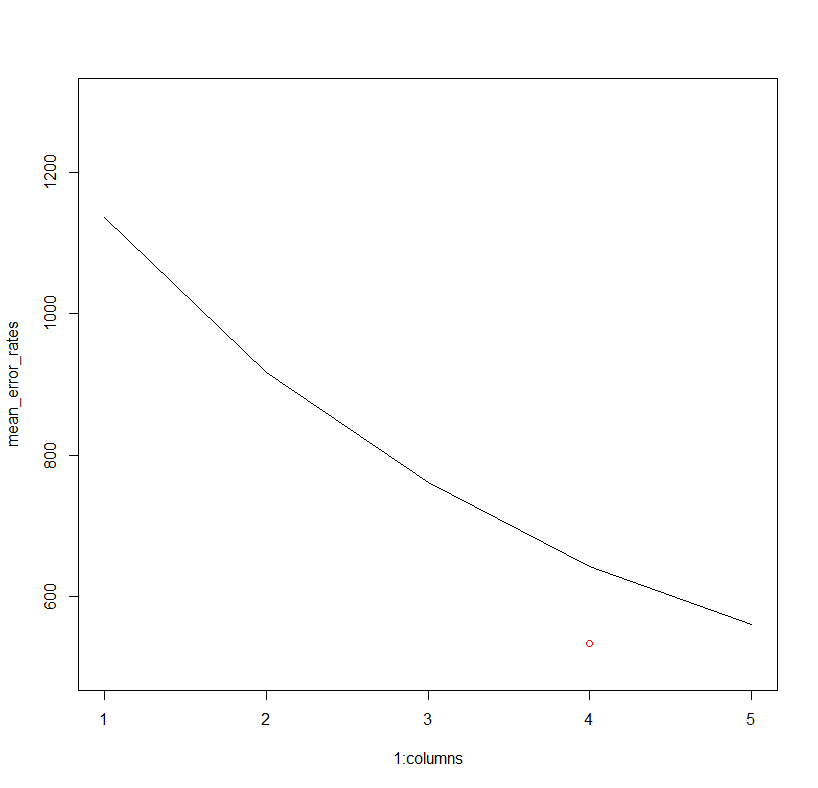
\includegraphics[width=\textwidth]{share/Lab2A1_me_features.png}  
        \caption{The mean error rate for different number of feature combinations.\label{fig:features} }
        \end{minipage}
        \end{figure}

        We can observe that the error rate decreases with the number of features selected, and the best possible chosen feature set contains: \emph{Agriculture, Education, Catholic, Infant Mortality}. For the next set of graphs shown below portrays the linear estimation of the features in the best feature subset. The model manages to approximate what humans would consider as the correct estimation.

        \begin{figure}[H]
        \centering
        \begin{minipage}[]{0.24\textwidth}
        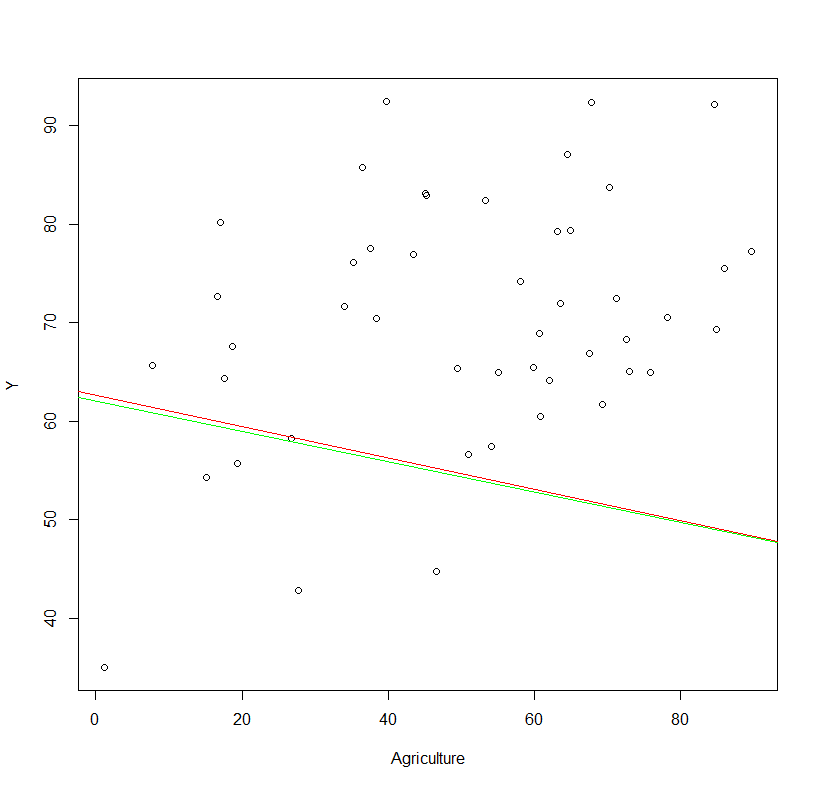
\includegraphics[width=\textwidth]{share/Lab2A1_lr_A.png}  
        \end{minipage}
        \begin{minipage}[]{0.24\textwidth}
        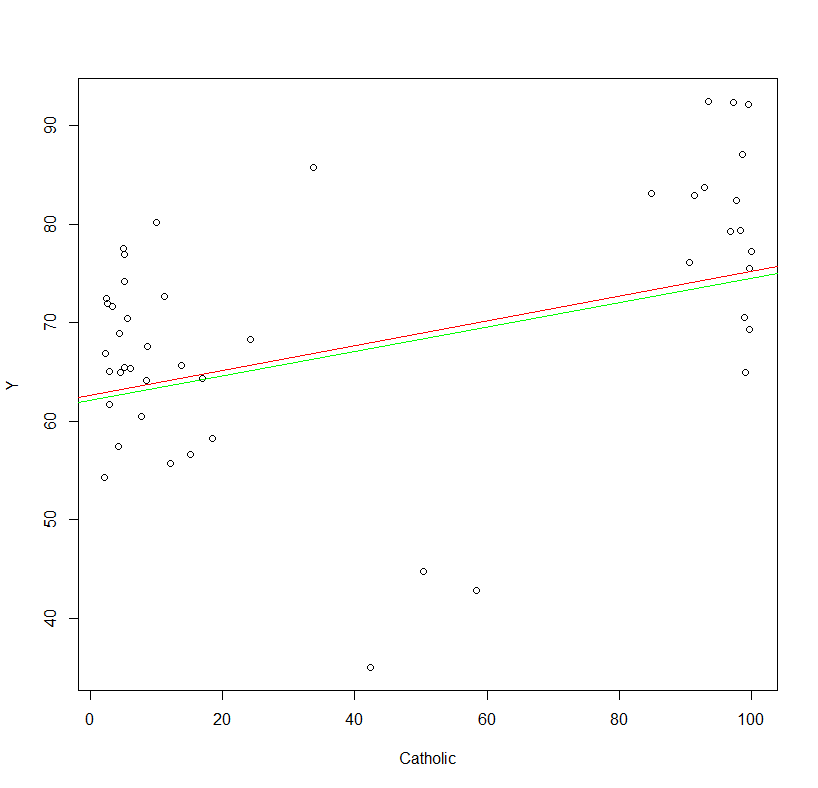
\includegraphics[width=\textwidth]{share/Lab2A1_lr_C.png}  
        \end{minipage}
        \begin{minipage}[]{0.24\textwidth}
        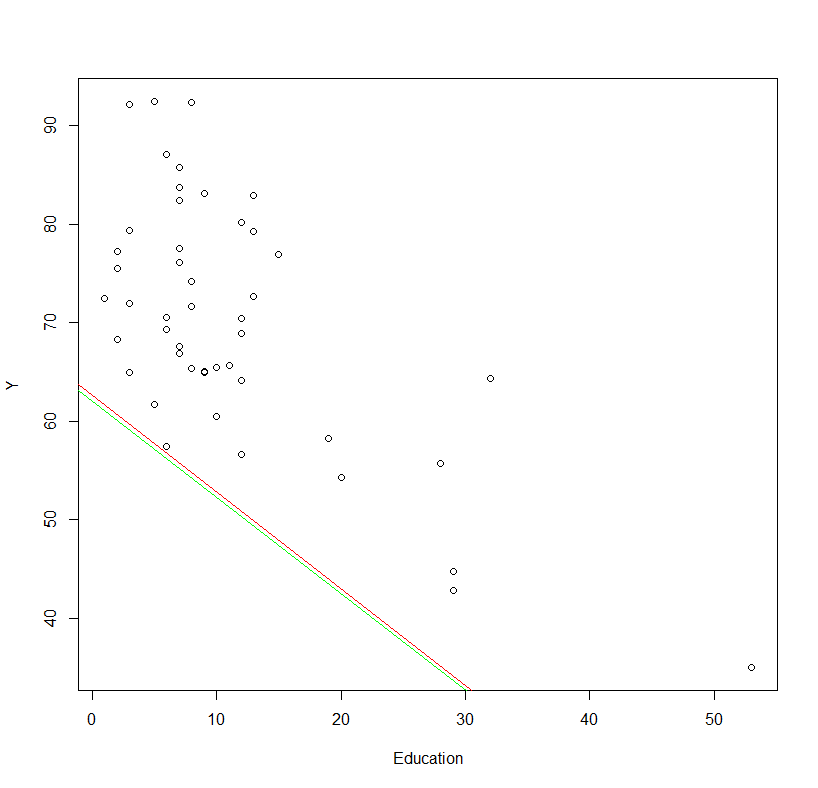
\includegraphics[width=\textwidth]{share/Lab2A1_lr_E.png}  
        \end{minipage}
        \begin{minipage}[]{0.24\textwidth}
        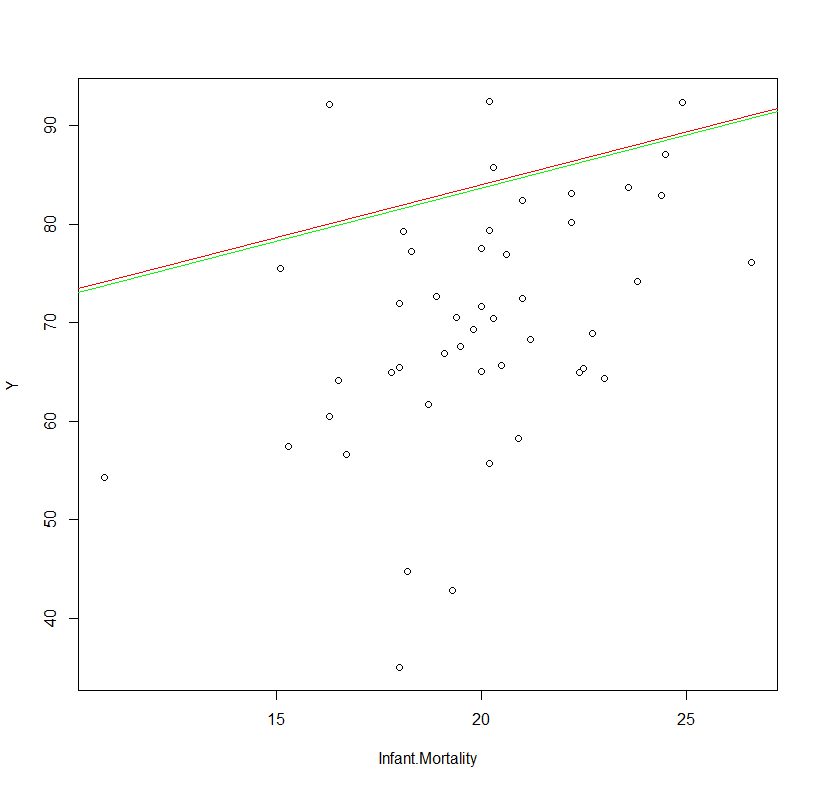
\includegraphics[width=\textwidth]{share/lab2A1_lr_IM.png}  
        \end{minipage}
        \end{figure}

    \section*{Assignment 2}
    It turns out moisture in meat might be correlated to the concentration of protein. The data given in the assignment yields a plot which has points densely located around a line. Meaning, it is rather clear that said statement is true since the points seem distributed linearly. The plot for this can be found in the Appendix. Assuming there is some linear model M that fits the data sufficiently well, one can might suspect that there is a model of higher polynomial order that fits it even better. The model can be described in the following manner: \(M_i \sim N(\sum_{j=0}^{i} w_{j} x^{i},\sigma^2)\). The assignment specifies that observations above polynomial order 6 is completely inadvisable in this context (only $M_{1 \mathrm{\ to\ } 6})$.

        \begin{figure}[H]
        \centering
        \begin{minipage}[]{0.5\textwidth}
        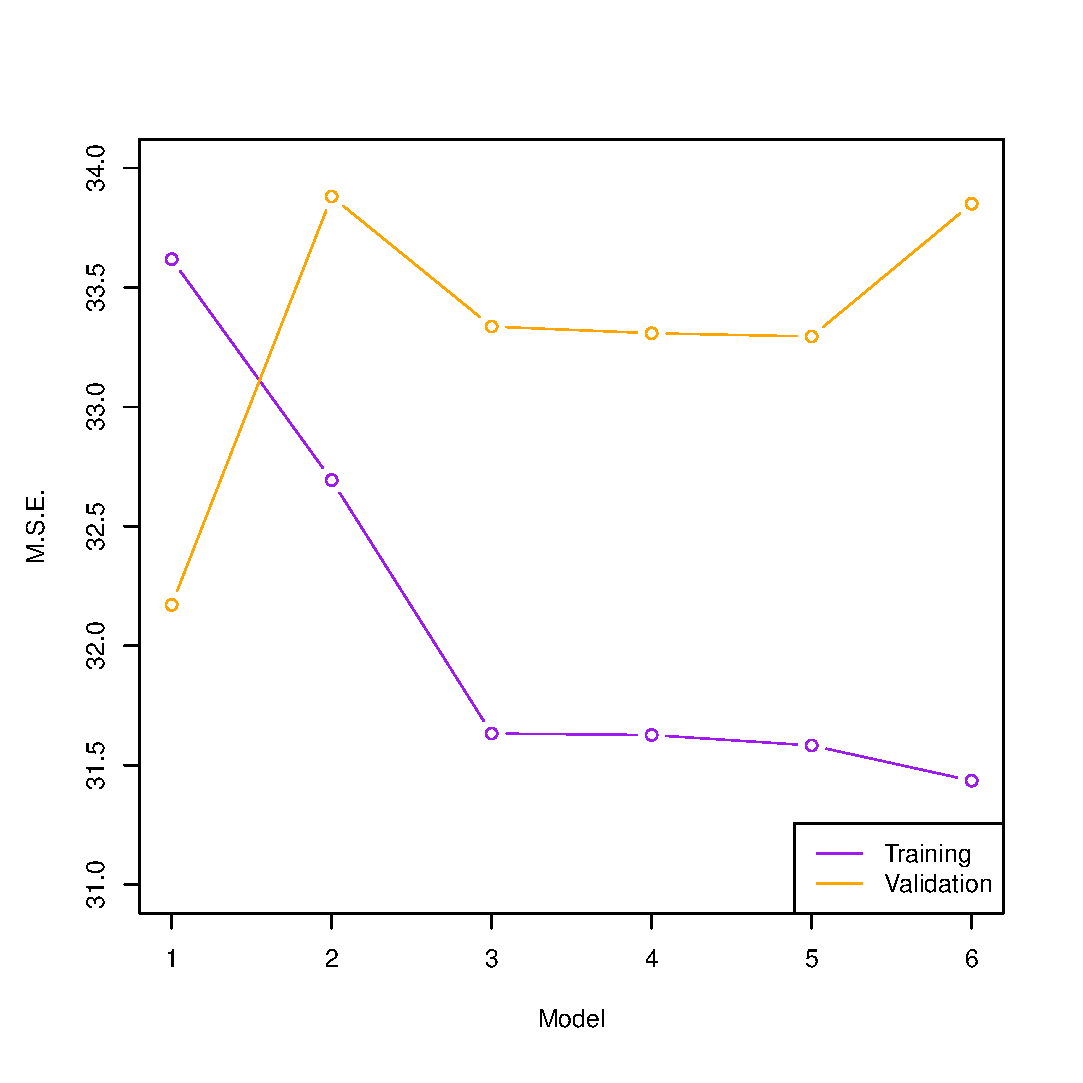
\includegraphics[width=\textwidth]{share/depends.eps}  
        \caption{The mean error rate for different number of feature combinations.\label{fig:depends} }
        \end{minipage}
        \end{figure}


        From the plot in figure \ref{fig:depends} the reader can observe that increasing the polynomial order leads to overfitting. This event is caused because though MSE for the training set decreases, the test set MSE is increasing. This means that any model \(M_i\) where $i > 1$, probably leads to worse predictions for the rest of the observation (not part of training data).

        The following explanations concerns how the input variables for Channels 1 - 100 correlates to Fat contents by doing variable selection using \texttt{stepAIC()}, which is a built-in \emph{R} function for doing this. \texttt{stepAIC()} works by constructing a model from removing and adding features to it. It starts the algorithm with the entire feature set, then removes one feature depending on a quantified representation of the model that takes into consideration its prediction accuracy as well as its necessity. One can define the direction of the algorithm, meaning it will only remove variables if one defines the direction as \emph{backwards}, and adding if it is defined as \emph{forward}, but using the \emph{both} keyword, they can be applied tougher. The \emph{both} keyword will result in a ``brute force'' solution which should elect the optimal set of features. By applying \texttt{stepAIC} to the dataset, where the feature set are \emph{Channel 1 - 100} and the response \emph{Fat}, the results were a staggering 64 features, where most were selected in the backwards part of the algorithm.

        Ridge regression works by taking into consideration the size of the parameters, this results in less variance for parameters since there are less options to choose from. By adding a representation of the size and factorize it by a \emph{penalty rate} ($\lambda$ in this case), one can control the importance of the size of parameters, meaning by increasing $\lambda$, it is more desirable for the algorithm to select such small parameters. This is done by adding the term $\sum_{i}{\mathbf{w}^2}$ to the usual \emph{OLS formula}. The library \emph{glmnet} provides such functionality. By setting the parameter $\lambda = 0.0$ (in \emph{glmnet()} that is), one can use \emph{Ridge regression} on the existing dataset. This yields Figure~\ref{fig:ridge}, as astute reader can observe, the coefficients converge uniformly towards zero, which is of course implied from the previously described explanation of Ridge (and also more graphically from Figure~\ref{fig:shape}).

    \begin{figure}[h!]
        \centering
        \caption{Ridge regression penalization.}
        \label{fig:ridge}
        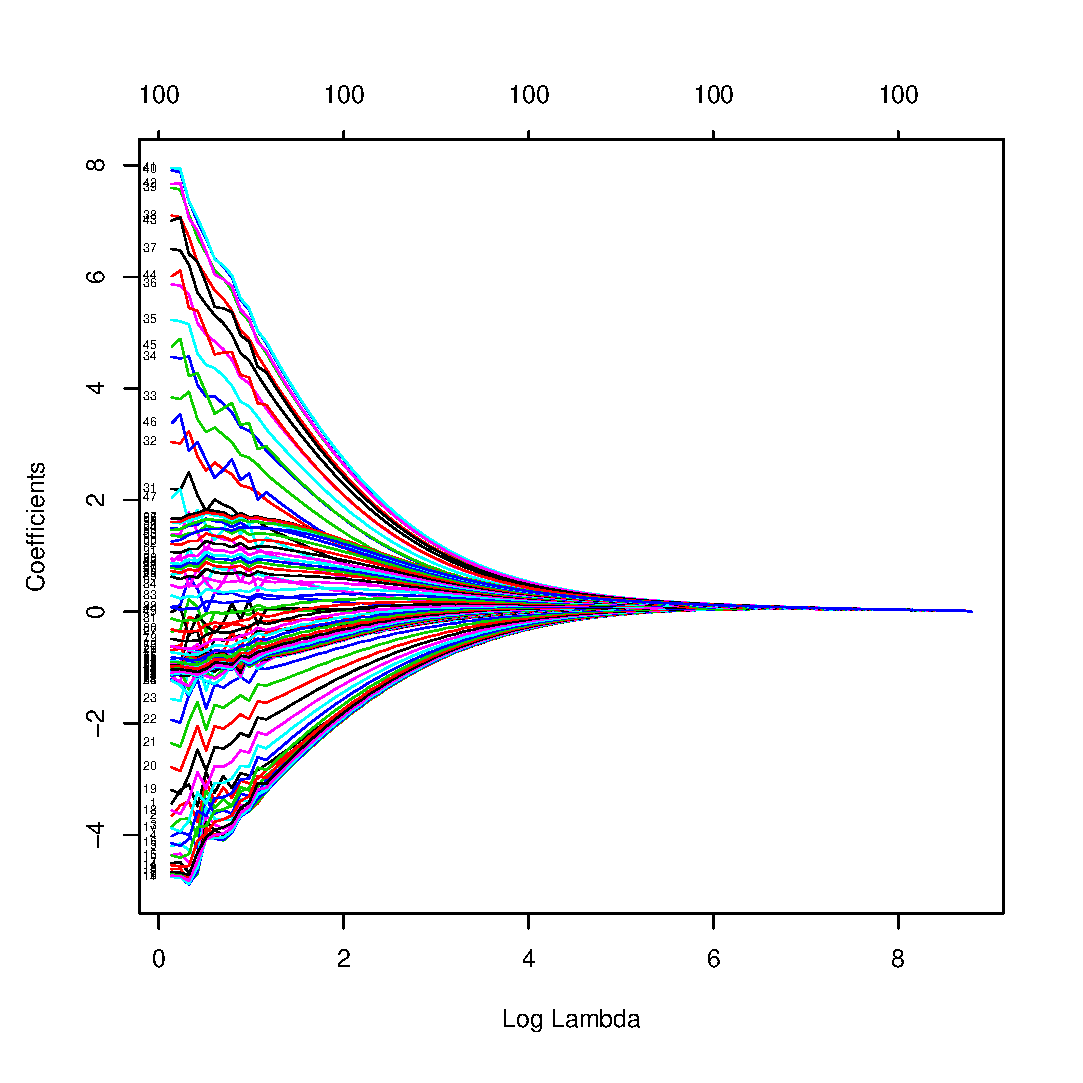
\includegraphics[width=0.35\textwidth]{share/ridge.eps}
    \end{figure}

        LASSO works similarly to Ridge, except that it represents the size of the parameters differently. Rather than using $\sum_{i}{\mathbf{w}^2}$ is uses $\sum_{i}{|\mathbf{w}|}$ instead. See Figure~\ref{fig:shape}. As can be seen, the edges are linear and there are four points where the distance from the origin is as large as possible, making at least one parameter zero. Because of this, LASSO converges individual parameters to zero faster than Ridge (instead of uniformly), this is because a tangent has to be parallel with the line from one extreme point to another (created from a feature), if it doesn't, the intersection will converge to an extreme point primarily. Thus, it excludes features in the model by assigning zero as a parameter. Practically, this can also be implemented by using \emph{glmnet}, this time by setting $\lambda = 1.0$. Figure~\ref{fig:lasso} confirms the previous assertions, the coefficients converge to zero not as uniformly as Ridge, in fact, they seem to converge individually (in an iterative fashion, after another).

    \begin{figure}[h!]
        \centering
        \caption{LASSO on the left, Ridge on the right. Distributed under the CC-license, created by \emph{Rezamohammadighazi} in LASSO on Wikipedia.}
        \label{fig:shape}
        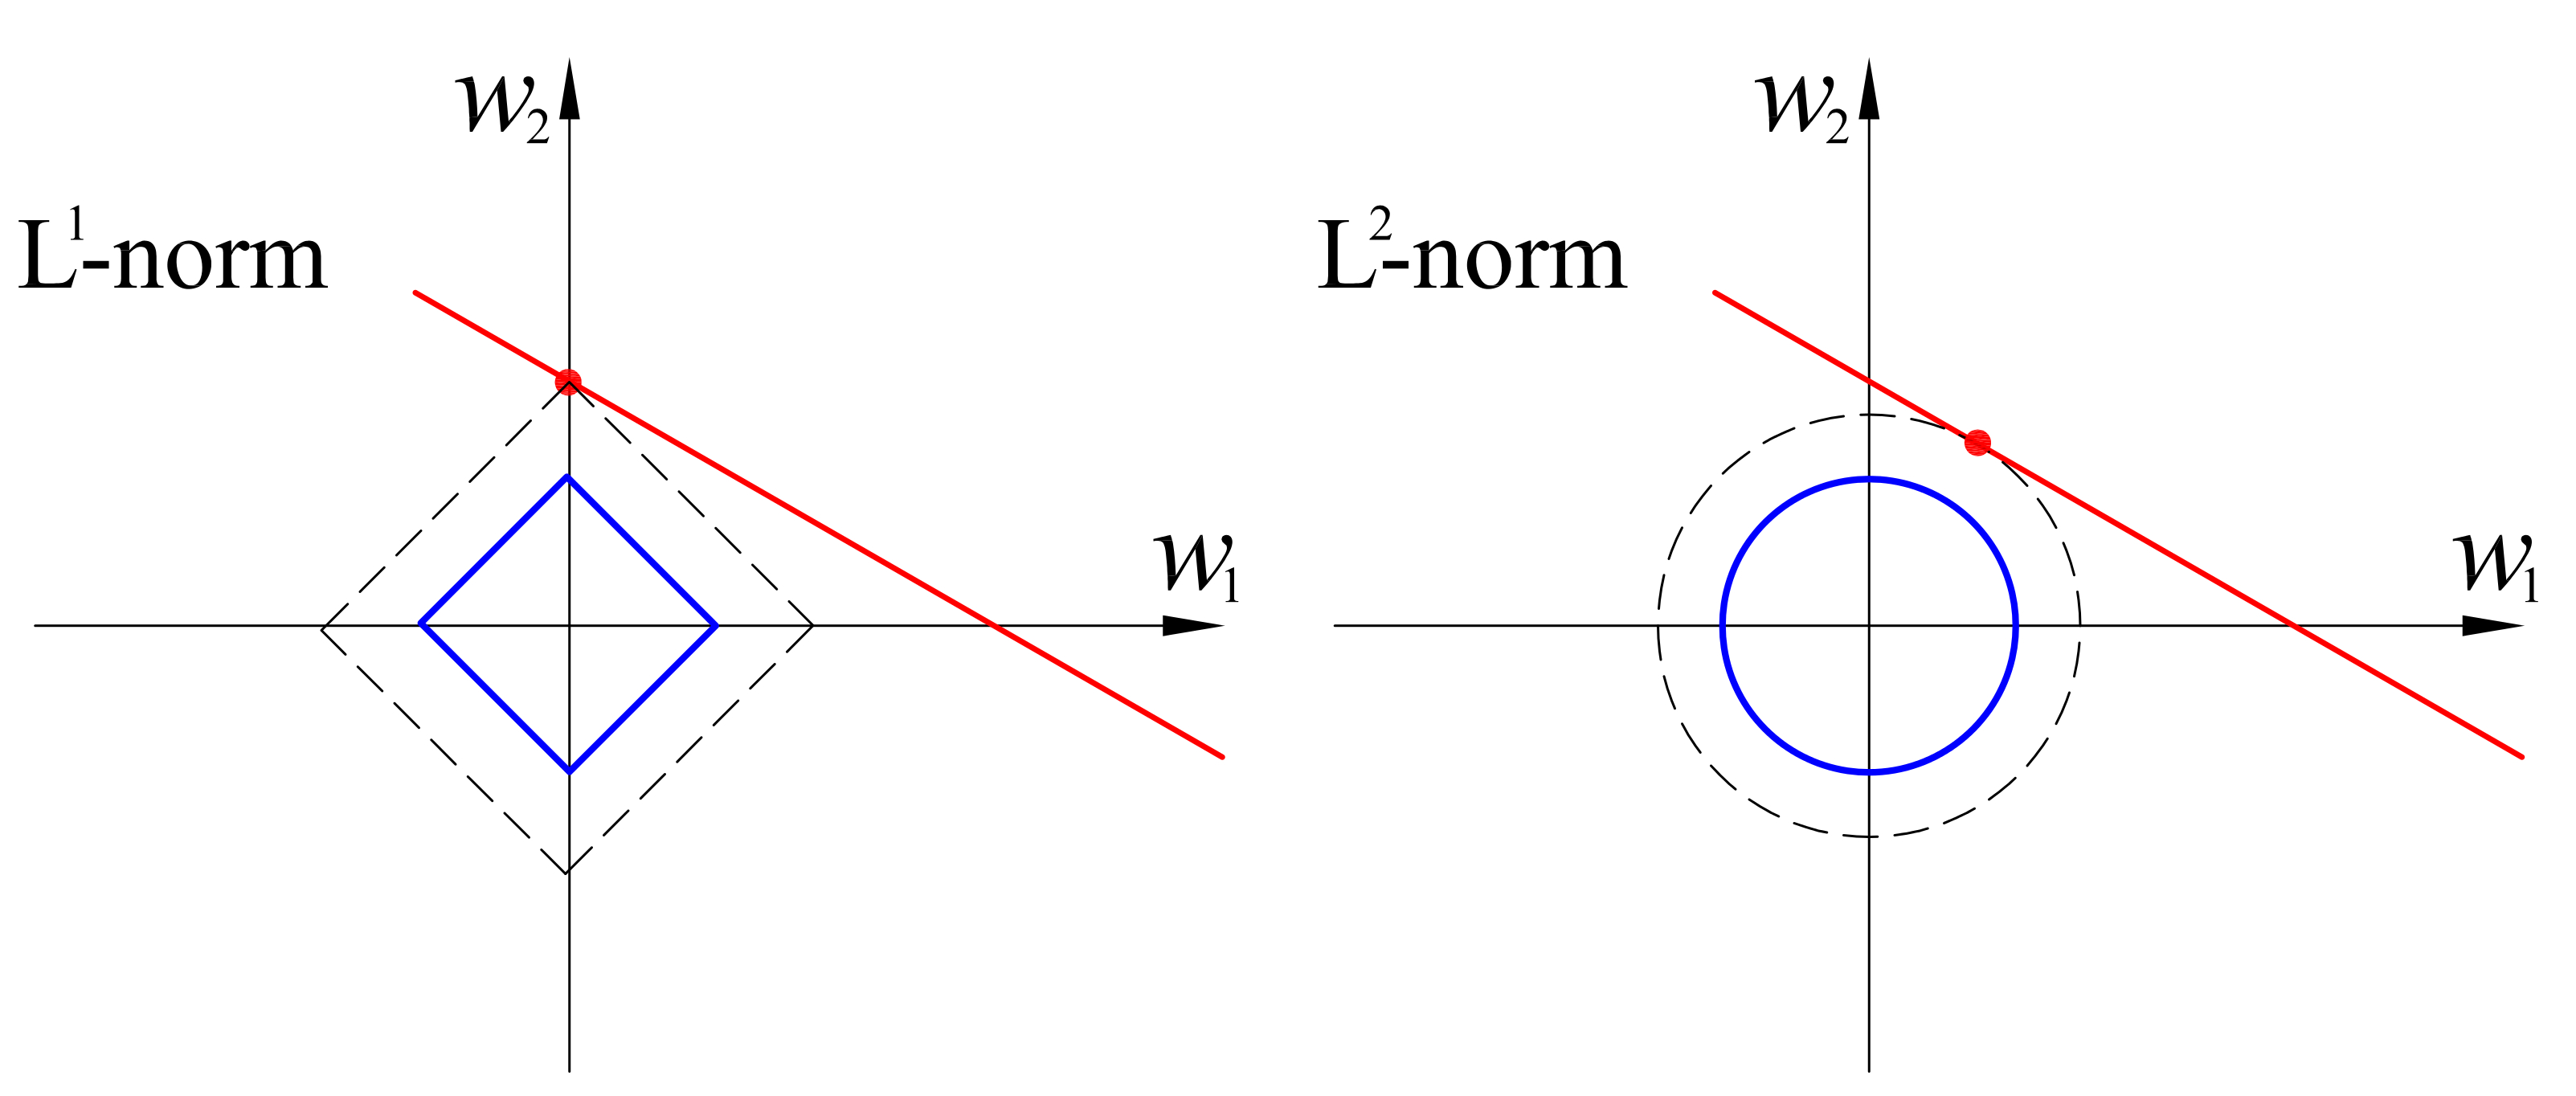
\includegraphics[width=0.35\textwidth]{share/shape.jpg}
    \end{figure}

    \begin{figure}[h!]
        \centering
        \caption{LASSO regression penalization.}
        \label{fig:lasso}
        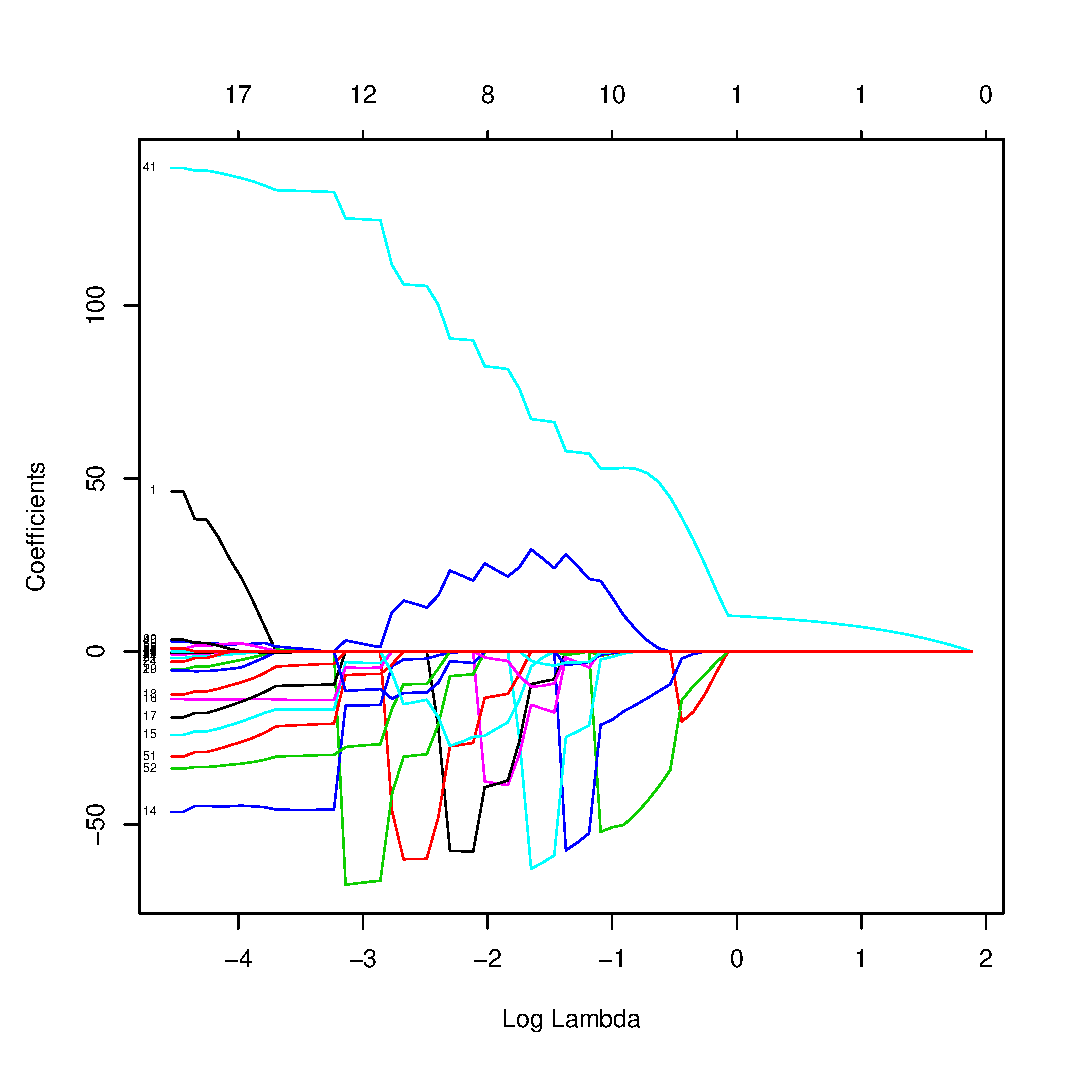
\includegraphics[width=0.35\textwidth]{share/lasso.eps}
    \end{figure}

        By using the built in \emph{k-fold cross-validation} algorithm in \emph{glmnet} for the \emph{Lasso model}, the best feature selection can be found. How \emph{k-fold cross-validation} work is explained back in Assignment 1. The best $\lambda$ has been reported to be around $0.029$ after running \texttt{cv.glmnet} for the same feature and response variables. Also, after plotting the \emph{log penalty} against the \emph{mean square error}, Figure~\ref{fig:kfold} is produced. As can be seen, the marked interval displays the best set of selected features, with their respective penalty values. The algorithm has selected 13 features, quite a few less than \emph{stepAIC}.

    \begin{figure}[h]
        \centering
        \caption{K-Fold Cross-Validation}
        \label{fig:kfold}
        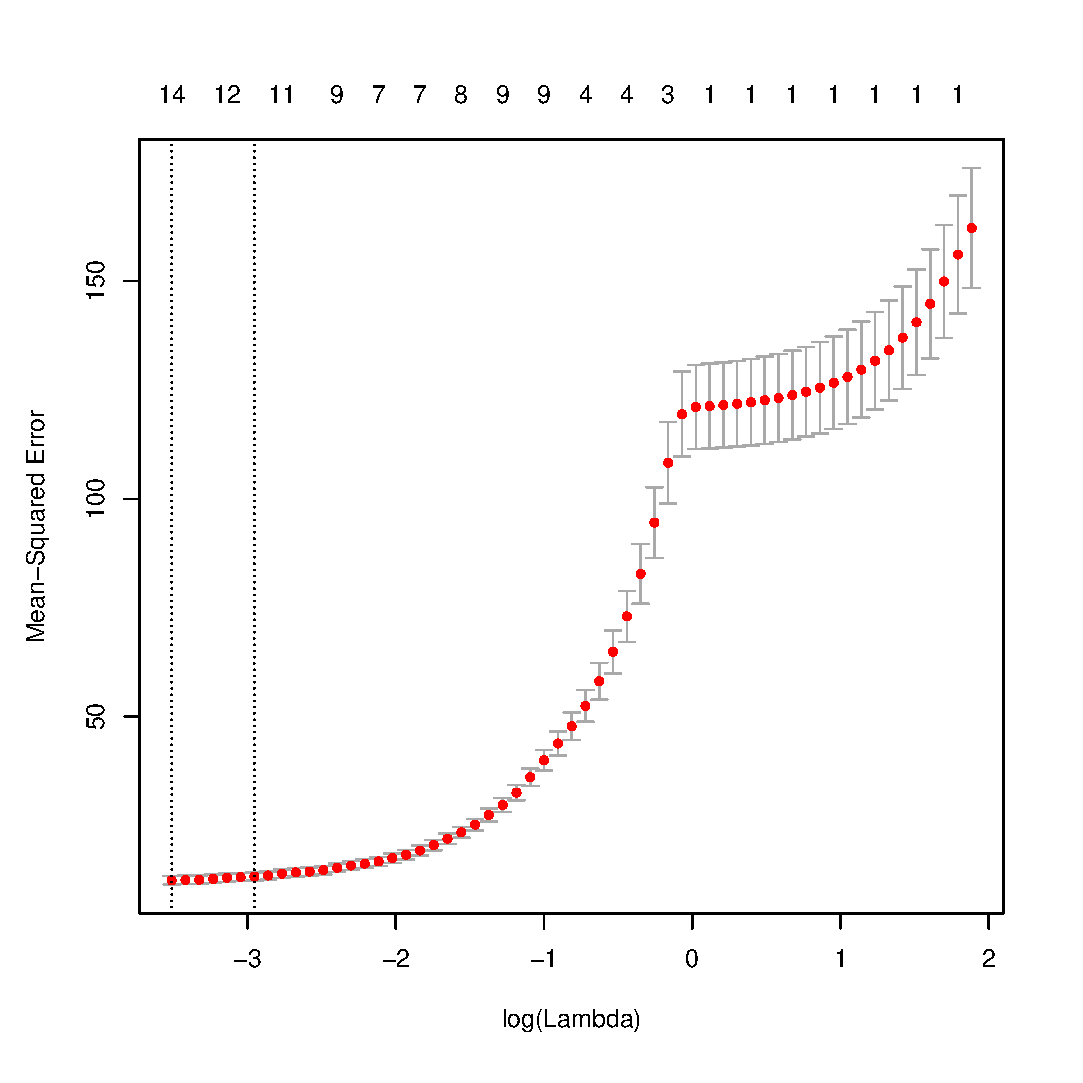
\includegraphics[width=0.35\textwidth]{share/kfold.eps}
    \end{figure}

    The results produced from \texttt{stepAIC()} gave 64 selected features, while \emph{k-fold cross-validation with the LASSO regression} produced only a set of 13 features. LASSO is more efficient when larger quantities of data are to be used when training a model, while \texttt{stepAIC()} will take longer to process but will in most cases result in a lower error rate value.

    \section*{Contributions}

    The written text has been contributed by all members of the group, where it was re-written from scratch together. However, certain plots, scripts and also algorithms were taken from certain individual reports. \emph{Erik} contributed with \emph{Algorithm 1} and some of the plots for \emph{Ridge} and \emph{Lasso} while \emph{Martin} contributed with most of the plots in Assignment 1 and also was chosen to provide the scripts for both assignments (to not have to piece together scripts, which was a hassle in past report). \emph{Sebastian} provided explanations on \emph{Ridge} \& \emph{Lasso}.

    \nocite{*} % No warnings.
    \bibliographystyle{alpha}
    \bibliography{report}
    \onecolumn \appendix
    \section*{Appendix}

    \lstinputlisting[caption={Script for Assignment 1},label={lst:assignment1}]{../share/script.r}
    \lstinputlisting[caption={Script for Assignment 2},label={lst:assignment2}]{../share/script2.r}

    \begin{figure}[h]
        \centering
        \caption{Moisture versus Protein}
        \label{fig:moistprot}
        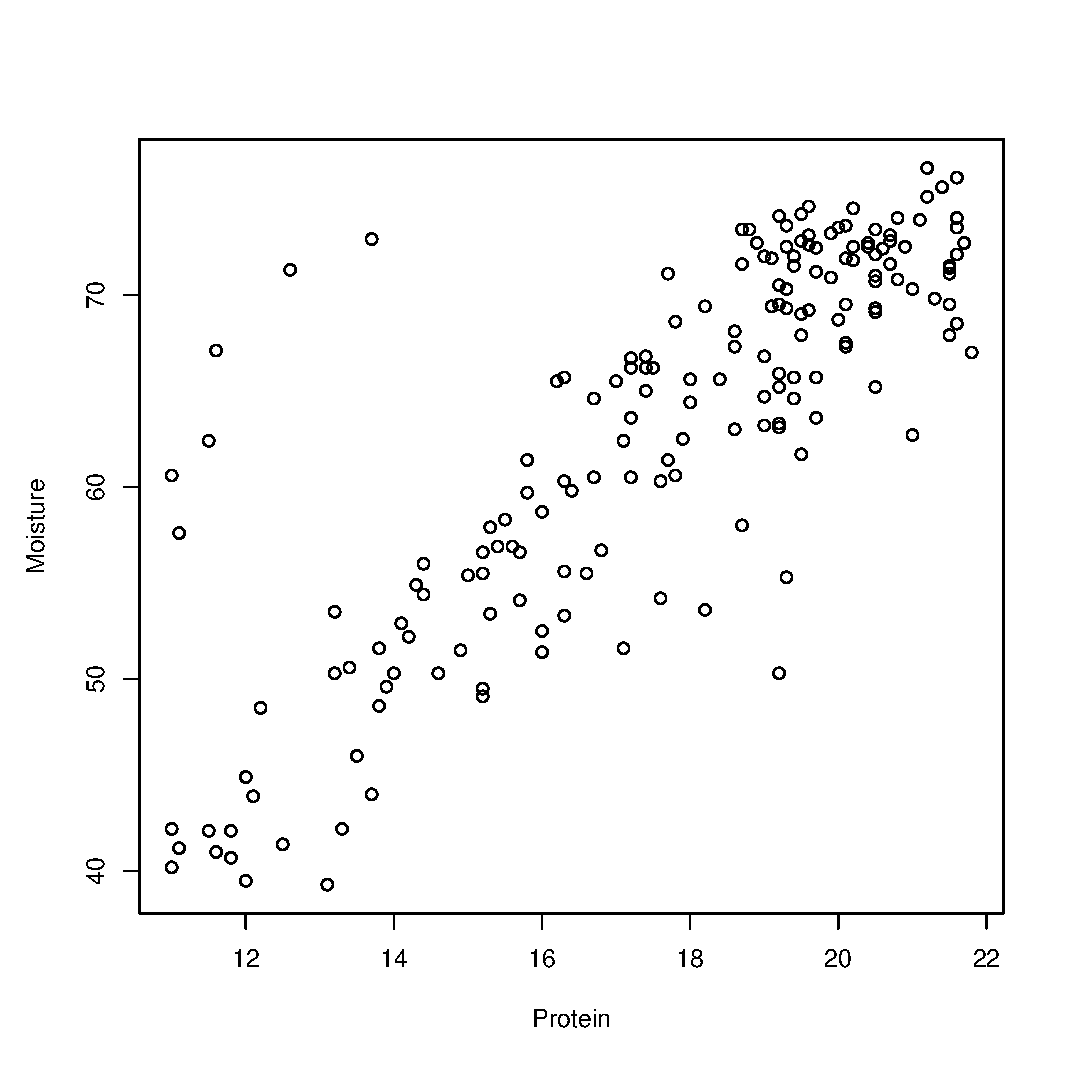
\includegraphics[width=0.35\textwidth]{share/linear.eps}
    \end{figure}

\end{document}
